\documentclass[]{article}
\usepackage{lmodern}
\usepackage{amssymb,amsmath}
\usepackage{ifxetex,ifluatex}
\usepackage{fixltx2e} % provides \textsubscript
\ifnum 0\ifxetex 1\fi\ifluatex 1\fi=0 % if pdftex
  \usepackage[T1]{fontenc}
  \usepackage[utf8]{inputenc}
\else % if luatex or xelatex
  \ifxetex
    \usepackage{mathspec}
  \else
    \usepackage{fontspec}
  \fi
  \defaultfontfeatures{Ligatures=TeX,Scale=MatchLowercase}
\fi
% use upquote if available, for straight quotes in verbatim environments
\IfFileExists{upquote.sty}{\usepackage{upquote}}{}
% use microtype if available
\IfFileExists{microtype.sty}{%
\usepackage{microtype}
\UseMicrotypeSet[protrusion]{basicmath} % disable protrusion for tt fonts
}{}
\usepackage[margin=1in]{geometry}
\usepackage{hyperref}
\hypersetup{unicode=true,
            pdftitle={MovieLens Rating Prediction Project},
            pdfauthor={Nabeel Khan},
            pdfborder={0 0 0},
            breaklinks=true}
\urlstyle{same}  % don't use monospace font for urls
\usepackage{color}
\usepackage{fancyvrb}
\newcommand{\VerbBar}{|}
\newcommand{\VERB}{\Verb[commandchars=\\\{\}]}
\DefineVerbatimEnvironment{Highlighting}{Verbatim}{commandchars=\\\{\}}
% Add ',fontsize=\small' for more characters per line
\usepackage{framed}
\definecolor{shadecolor}{RGB}{248,248,248}
\newenvironment{Shaded}{\begin{snugshade}}{\end{snugshade}}
\newcommand{\AlertTok}[1]{\textcolor[rgb]{0.94,0.16,0.16}{#1}}
\newcommand{\AnnotationTok}[1]{\textcolor[rgb]{0.56,0.35,0.01}{\textbf{\textit{#1}}}}
\newcommand{\AttributeTok}[1]{\textcolor[rgb]{0.77,0.63,0.00}{#1}}
\newcommand{\BaseNTok}[1]{\textcolor[rgb]{0.00,0.00,0.81}{#1}}
\newcommand{\BuiltInTok}[1]{#1}
\newcommand{\CharTok}[1]{\textcolor[rgb]{0.31,0.60,0.02}{#1}}
\newcommand{\CommentTok}[1]{\textcolor[rgb]{0.56,0.35,0.01}{\textit{#1}}}
\newcommand{\CommentVarTok}[1]{\textcolor[rgb]{0.56,0.35,0.01}{\textbf{\textit{#1}}}}
\newcommand{\ConstantTok}[1]{\textcolor[rgb]{0.00,0.00,0.00}{#1}}
\newcommand{\ControlFlowTok}[1]{\textcolor[rgb]{0.13,0.29,0.53}{\textbf{#1}}}
\newcommand{\DataTypeTok}[1]{\textcolor[rgb]{0.13,0.29,0.53}{#1}}
\newcommand{\DecValTok}[1]{\textcolor[rgb]{0.00,0.00,0.81}{#1}}
\newcommand{\DocumentationTok}[1]{\textcolor[rgb]{0.56,0.35,0.01}{\textbf{\textit{#1}}}}
\newcommand{\ErrorTok}[1]{\textcolor[rgb]{0.64,0.00,0.00}{\textbf{#1}}}
\newcommand{\ExtensionTok}[1]{#1}
\newcommand{\FloatTok}[1]{\textcolor[rgb]{0.00,0.00,0.81}{#1}}
\newcommand{\FunctionTok}[1]{\textcolor[rgb]{0.00,0.00,0.00}{#1}}
\newcommand{\ImportTok}[1]{#1}
\newcommand{\InformationTok}[1]{\textcolor[rgb]{0.56,0.35,0.01}{\textbf{\textit{#1}}}}
\newcommand{\KeywordTok}[1]{\textcolor[rgb]{0.13,0.29,0.53}{\textbf{#1}}}
\newcommand{\NormalTok}[1]{#1}
\newcommand{\OperatorTok}[1]{\textcolor[rgb]{0.81,0.36,0.00}{\textbf{#1}}}
\newcommand{\OtherTok}[1]{\textcolor[rgb]{0.56,0.35,0.01}{#1}}
\newcommand{\PreprocessorTok}[1]{\textcolor[rgb]{0.56,0.35,0.01}{\textit{#1}}}
\newcommand{\RegionMarkerTok}[1]{#1}
\newcommand{\SpecialCharTok}[1]{\textcolor[rgb]{0.00,0.00,0.00}{#1}}
\newcommand{\SpecialStringTok}[1]{\textcolor[rgb]{0.31,0.60,0.02}{#1}}
\newcommand{\StringTok}[1]{\textcolor[rgb]{0.31,0.60,0.02}{#1}}
\newcommand{\VariableTok}[1]{\textcolor[rgb]{0.00,0.00,0.00}{#1}}
\newcommand{\VerbatimStringTok}[1]{\textcolor[rgb]{0.31,0.60,0.02}{#1}}
\newcommand{\WarningTok}[1]{\textcolor[rgb]{0.56,0.35,0.01}{\textbf{\textit{#1}}}}
\usepackage{longtable,booktabs}
\usepackage{graphicx,grffile}
\makeatletter
\def\maxwidth{\ifdim\Gin@nat@width>\linewidth\linewidth\else\Gin@nat@width\fi}
\def\maxheight{\ifdim\Gin@nat@height>\textheight\textheight\else\Gin@nat@height\fi}
\makeatother
% Scale images if necessary, so that they will not overflow the page
% margins by default, and it is still possible to overwrite the defaults
% using explicit options in \includegraphics[width, height, ...]{}
\setkeys{Gin}{width=\maxwidth,height=\maxheight,keepaspectratio}
\IfFileExists{parskip.sty}{%
\usepackage{parskip}
}{% else
\setlength{\parindent}{0pt}
\setlength{\parskip}{6pt plus 2pt minus 1pt}
}
\setlength{\emergencystretch}{3em}  % prevent overfull lines
\providecommand{\tightlist}{%
  \setlength{\itemsep}{0pt}\setlength{\parskip}{0pt}}
\setcounter{secnumdepth}{5}
% Redefines (sub)paragraphs to behave more like sections
\ifx\paragraph\undefined\else
\let\oldparagraph\paragraph
\renewcommand{\paragraph}[1]{\oldparagraph{#1}\mbox{}}
\fi
\ifx\subparagraph\undefined\else
\let\oldsubparagraph\subparagraph
\renewcommand{\subparagraph}[1]{\oldsubparagraph{#1}\mbox{}}
\fi

%%% Use protect on footnotes to avoid problems with footnotes in titles
\let\rmarkdownfootnote\footnote%
\def\footnote{\protect\rmarkdownfootnote}

%%% Change title format to be more compact
\usepackage{titling}

% Create subtitle command for use in maketitle
\providecommand{\subtitle}[1]{
  \posttitle{
    \begin{center}\large#1\end{center}
    }
}

\setlength{\droptitle}{-2em}

  \title{MovieLens Rating Prediction Project}
    \pretitle{\vspace{\droptitle}\centering\huge}
  \posttitle{\par}
    \author{Nabeel Khan}
    \preauthor{\centering\large\emph}
  \postauthor{\par}
      \predate{\centering\large\emph}
  \postdate{\par}
    \date{21-May-2020}


\begin{document}
\maketitle

{
\setcounter{tocdepth}{2}
\tableofcontents
}
\section{Introduction} 
\label{sec:introduction}

This report is part of the `HarvardX: PH125.9x Data Science: Capstone'
course. In this report, we discuss various approaches to develop a
recommender system using the acquired data science skills.

\subsection{Background} 
\label{sec:background}

The recommender systems predict the interests of users and recommend
product items that are quite likely interesting for
them\cite{rsystems,rsystems1}. The recommender systems use state of the
art machine learning algorithms to make precise predictions. The
recommender systems are commonly used by Netflix, YouTube, Spotify,
Amazon, or Ebay.

One of the famous success stories of the recommender system is Netflix
competition \cite{nfc}. In 2006, Netflix announced the awarding of one
million dollar prize to a team, which can come up with the best
filtering algorithm to predict user ratings for movies based on previous
ratings. It took three years for a team to win the competition. The
winning team improved the accuracy of the Netflix recommender system by
10\%.

\subsection{Aim of Project} 
\label{sec:projectaim}

This project aims to develop a recommender system using a model to
predict movie ratings based on suitable predictors.

\section{Dataset and Evaluation Metric} 
\label{sec:datasetmetric}

Netflix dataset is not available online. So, we use the 10M version of
MoiveLens dataset in this project \cite{dataset}. The dataset is
generated by the GroupLens, which is a research lab in the Department of
Computer Science and Engineering at the University of Minnesota. The
dataset contains 10 million ratings. We will split the data into
training and validation sets to develop our model.

To evaluate the performance of the model, we will use Root Mean Square
Error (RMSE) \cite{rmse} as defined in Equation \ref{eq:rmse}. The RMSE
is a standard method to measure the error of a model in predicting
quantitative data.

\begin{equation}
\label{eq:rmse}
RMSE = \sqrt{\frac{1}{n}\displaystyle\sum_{i=1}^{n} (\hat{y}_{i}-y_{i})^{2}}
\end{equation}

Where \(\hat{y}_{i}\) refers to the predicted values by the model,
\({y}_{i}\) refers to the actual values, and \emph{n} refers to the
total number of observations. The RMSE is a commonly used metric for
analyzing the performance of models, but it can produce biased results
in the presence of a large number of outliers or noise in the data. In
this project, the RMSE will indicate how close model predictions are to
the actual ratings in the validation set.

\subsection{Download Data}
\label{datadownload}

We download data from the website. Then, we split data into a training
set referred to as \emph{edx}, and test set referred to as
\emph{validation}. 10\% of the data is used for validation, and 90\% is
used for training.

\begin{itemize}
\item The model is trained using \emph{edx} dataset, and 
we compute RMSE using \emph{validation} dataset.
\end{itemize}

\begin{Shaded}
\begin{Highlighting}[]
\CommentTok{################################}
\CommentTok{#  Install packages (if not installed)}
\CommentTok{################################}
\CommentTok{# Note: this process could take a couple of minutes}
\NormalTok{repos_path<-}\StringTok{ "http://cran.us.r-project.org"}
\ControlFlowTok{if}\NormalTok{(}\OperatorTok{!}\KeywordTok{require}\NormalTok{(tidyverse)) }\KeywordTok{install.packages}\NormalTok{(}\StringTok{"tidyverse"}\NormalTok{, }\DataTypeTok{repos =}\NormalTok{repos_path)}
\end{Highlighting}
\end{Shaded}

\begin{verbatim}
## Loading required package: tidyverse
\end{verbatim}

\begin{verbatim}
## -- Attaching packages ---------------------------------------------------- tidyverse 1.2.1 --
\end{verbatim}

\begin{verbatim}
## v ggplot2 3.2.1     v purrr   0.3.3
## v tibble  2.1.3     v dplyr   0.8.3
## v tidyr   1.0.0     v stringr 1.4.0
## v readr   1.3.1     v forcats 0.4.0
\end{verbatim}

\begin{verbatim}
## -- Conflicts ------------------------------------------------------- tidyverse_conflicts() --
## x dplyr::filter() masks stats::filter()
## x dplyr::lag()    masks stats::lag()
\end{verbatim}

\begin{Shaded}
\begin{Highlighting}[]
\ControlFlowTok{if}\NormalTok{(}\OperatorTok{!}\KeywordTok{require}\NormalTok{(caret)) }\KeywordTok{install.packages}\NormalTok{(}\StringTok{"caret"}\NormalTok{, }\DataTypeTok{repos =}\NormalTok{ repos_path)}
\end{Highlighting}
\end{Shaded}

\begin{verbatim}
## Loading required package: caret
\end{verbatim}

\begin{verbatim}
## Warning: package 'caret' was built under R version 3.6.3
\end{verbatim}

\begin{verbatim}
## Loading required package: lattice
\end{verbatim}

\begin{verbatim}
## 
## Attaching package: 'caret'
\end{verbatim}

\begin{verbatim}
## The following object is masked from 'package:purrr':
## 
##     lift
\end{verbatim}

\begin{Shaded}
\begin{Highlighting}[]
\ControlFlowTok{if}\NormalTok{(}\OperatorTok{!}\KeywordTok{require}\NormalTok{(data.table)) }\KeywordTok{install.packages}\NormalTok{(}\StringTok{"data.table"}\NormalTok{, }\DataTypeTok{repos =}\NormalTok{repos_path)}
\end{Highlighting}
\end{Shaded}

\begin{verbatim}
## Loading required package: data.table
\end{verbatim}

\begin{verbatim}
## Warning: package 'data.table' was built under R version 3.6.3
\end{verbatim}

\begin{verbatim}
## 
## Attaching package: 'data.table'
\end{verbatim}

\begin{verbatim}
## The following objects are masked from 'package:dplyr':
## 
##     between, first, last
\end{verbatim}

\begin{verbatim}
## The following object is masked from 'package:purrr':
## 
##     transpose
\end{verbatim}

\begin{Shaded}
\begin{Highlighting}[]
\ControlFlowTok{if}\NormalTok{(}\OperatorTok{!}\KeywordTok{require}\NormalTok{(lubridate)) }\KeywordTok{install.packages}\NormalTok{(}\StringTok{"lubridate"}\NormalTok{, }\DataTypeTok{repos =}\NormalTok{ repos_path)}
\end{Highlighting}
\end{Shaded}

\begin{verbatim}
## Loading required package: lubridate
\end{verbatim}

\begin{verbatim}
## 
## Attaching package: 'lubridate'
\end{verbatim}

\begin{verbatim}
## The following objects are masked from 'package:data.table':
## 
##     hour, isoweek, mday, minute, month, quarter, second, wday,
##     week, yday, year
\end{verbatim}

\begin{verbatim}
## The following object is masked from 'package:base':
## 
##     date
\end{verbatim}

\begin{Shaded}
\begin{Highlighting}[]
\ControlFlowTok{if}\NormalTok{(}\OperatorTok{!}\KeywordTok{require}\NormalTok{(dplyr)) }\KeywordTok{install.packages}\NormalTok{(}\StringTok{"dplyr"}\NormalTok{, }\DataTypeTok{repos =}\NormalTok{ repos_path)}
\ControlFlowTok{if}\NormalTok{(}\OperatorTok{!}\KeywordTok{require}\NormalTok{(sjmisc)) }\KeywordTok{install.packages}\NormalTok{(}\StringTok{"dplyr"}\NormalTok{, }\DataTypeTok{repos =}\NormalTok{ repos_path)}
\end{Highlighting}
\end{Shaded}

\begin{verbatim}
## Loading required package: sjmisc
\end{verbatim}

\begin{verbatim}
## Warning: package 'sjmisc' was built under R version 3.6.3
\end{verbatim}

\begin{verbatim}
## 
## Attaching package: 'sjmisc'
\end{verbatim}

\begin{verbatim}
## The following object is masked from 'package:purrr':
## 
##     is_empty
\end{verbatim}

\begin{verbatim}
## The following object is masked from 'package:tidyr':
## 
##     replace_na
\end{verbatim}

\begin{verbatim}
## The following object is masked from 'package:tibble':
## 
##     add_case
\end{verbatim}

\begin{Shaded}
\begin{Highlighting}[]
\CommentTok{################################}
\CommentTok{# Load libraries}
\CommentTok{################################}
\KeywordTok{library}\NormalTok{(lubridate)}
\KeywordTok{library}\NormalTok{(tidyverse)}
\KeywordTok{library}\NormalTok{(dplyr)}
\KeywordTok{library}\NormalTok{(lubridate)}
\KeywordTok{library}\NormalTok{(sjmisc)}
\end{Highlighting}
\end{Shaded}

\begin{Shaded}
\begin{Highlighting}[]
\CommentTok{################################}
\CommentTok{# Downloading data}
\CommentTok{################################}
\CommentTok{# MovieLens 10M dataset:}
 \CommentTok{# https://grouplens.org/datasets/movielens/10m/}
 \CommentTok{# http://files.grouplens.org/datasets/movielens/ml-10m.zip}

\NormalTok{url <-}\StringTok{ "http://files.grouplens.org/datasets/movielens/ml-10m.zip"}
\NormalTok{dl <-}\StringTok{ }\KeywordTok{tempfile}\NormalTok{()}
    \KeywordTok{download.file}\NormalTok{(url, dl)}
  
\NormalTok{ratings <-}\StringTok{ }\KeywordTok{fread}\NormalTok{(}\DataTypeTok{text =} \KeywordTok{gsub}\NormalTok{(}\StringTok{"::"}\NormalTok{, }\StringTok{"}\CharTok{\textbackslash{}t}\StringTok{"}\NormalTok{, }\KeywordTok{readLines}\NormalTok{(}\KeywordTok{unzip}\NormalTok{(dl, }\StringTok{"ml-10M100K/ratings.dat"}\NormalTok{))), }\DataTypeTok{col.names =} \KeywordTok{c}\NormalTok{(}\StringTok{"userId"}\NormalTok{, }\StringTok{"movieId"}\NormalTok{, }\StringTok{"rating"}\NormalTok{, }\StringTok{"timestamp"}\NormalTok{))}
\NormalTok{movies <-}\StringTok{ }\KeywordTok{str_split_fixed}\NormalTok{(}\KeywordTok{readLines}\NormalTok{(}\KeywordTok{unzip}\NormalTok{(dl, }\StringTok{"ml-10M100K/movies.dat"}\NormalTok{)), }\StringTok{"}\CharTok{\textbackslash{}\textbackslash{}}\StringTok{::"}\NormalTok{, }\DecValTok{3}\NormalTok{)}
   \KeywordTok{colnames}\NormalTok{(movies) <-}\StringTok{ }\KeywordTok{c}\NormalTok{(}\StringTok{"movieId"}\NormalTok{, }\StringTok{"title"}\NormalTok{, }\StringTok{"genres"}\NormalTok{)}
\NormalTok{   movies <-}\StringTok{ }\KeywordTok{as.data.frame}\NormalTok{(movies) }\OperatorTok\StringTok{ }\KeywordTok{mutate}\NormalTok{(}\DataTypeTok{movieId =}   \KeywordTok{as.numeric}\NormalTok{(}\KeywordTok{levels}\NormalTok{(movieId))[movieId], }\DataTypeTok{title =} \KeywordTok{as.character}\NormalTok{(title), }\DataTypeTok{genres =}    \KeywordTok{as.character}\NormalTok{(genres))}

\CommentTok{################################}
\CommentTok{# Creating edx and validation sets}
\CommentTok{################################}
\NormalTok{movielens <-}\StringTok{ }\KeywordTok{left_join}\NormalTok{(ratings, movies, }\DataTypeTok{by =} \StringTok{"movieId"}\NormalTok{)}


\CommentTok{# Validation set will be 10% of MovieLens data}
\KeywordTok{set.seed}\NormalTok{(}\DecValTok{1}\NormalTok{, }\DataTypeTok{sample.kind =} \StringTok{"Rounding"}\NormalTok{)}
\end{Highlighting}
\end{Shaded}

\begin{verbatim}
## Warning in set.seed(1, sample.kind = "Rounding"): non-uniform 'Rounding'
## sampler used
\end{verbatim}

\begin{Shaded}
\begin{Highlighting}[]
\NormalTok{test_index <-}\StringTok{ }\KeywordTok{createDataPartition}\NormalTok{(}\DataTypeTok{y =}\NormalTok{ movielens}\OperatorTok{$}\NormalTok{rating, }\DataTypeTok{times =} \DecValTok{1}\NormalTok{, }\DataTypeTok{p =} \FloatTok{0.1}\NormalTok{, }\DataTypeTok{list =} \OtherTok{FALSE}\NormalTok{)}

\NormalTok{edx <-}\StringTok{ }\NormalTok{movielens[}\OperatorTok{-}\NormalTok{test_index,]}
\NormalTok{temp <-}\StringTok{ }\NormalTok{movielens[test_index,]}

\CommentTok{# Make sure userId and movieId in validation set are also in edx set}
\NormalTok{validation <-}\StringTok{ }\NormalTok{temp }\OperatorTok\StringTok{ }
\StringTok{      }\KeywordTok{semi_join}\NormalTok{(edx, }\DataTypeTok{by =} \StringTok{"movieId"}\NormalTok{) }\OperatorTok
\StringTok{      }\KeywordTok{semi_join}\NormalTok{(edx, }\DataTypeTok{by =} \StringTok{"userId"}\NormalTok{)}

\CommentTok{# Add rows removed from validation set back into edx set}
\NormalTok{removed <-}\StringTok{ }\KeywordTok{anti_join}\NormalTok{(temp, validation)}
\end{Highlighting}
\end{Shaded}

\begin{verbatim}
## Joining, by = c("userId", "movieId", "rating", "timestamp", "title", "genres")
\end{verbatim}

\begin{Shaded}
\begin{Highlighting}[]
\NormalTok{ edx <-}\StringTok{ }\KeywordTok{rbind}\NormalTok{(edx, removed)}

 \CommentTok{# Removing the objects from environment as no longer required}
\KeywordTok{rm}\NormalTok{(dl, ratings, movies, test_index, temp, movielens, removed)}
\end{Highlighting}
\end{Shaded}

\section{Data Exploration}
\label{sec:dataexploration}

In this section, we explore the dataset to get familiar with it. We also
perform some data wrangling. Data wrangling is the process of cleaning,
structuring, or enriching raw data into the desired format to make
better decisions and get meaningful insights.

The dataset contains six variables namely \texttt{userID",}movieID``,
\texttt{rating",}timestamp'',
\texttt{title\textquotesingle{}",\ and}genres``. The ``timestamp''
indicates the date on which a user recorded his reviews for a particular
movie. Each row in the dataset represents a single rating of a user for
a single movie.

\begin{Shaded}
\begin{Highlighting}[]
\KeywordTok{head}\NormalTok{(edx)}
\end{Highlighting}
\end{Shaded}

\begin{longtable}[]{@{}lrrrrll@{}}
\toprule
& userId & movieId & rating & timestamp & title & genres\tabularnewline
\midrule
\endhead
1 & 1 & 122 & 5 & 838985046 & Boomerang (1992) &
Comedy\textbar Romance\tabularnewline
2 & 1 & 185 & 5 & 838983525 & Net, The (1995) &
Action\textbar Crime\textbar Thriller\tabularnewline
4 & 1 & 292 & 5 & 838983421 & Outbreak (1995) &
Action\textbar Drama\textbar Sci-Fi\textbar Thriller\tabularnewline
5 & 1 & 316 & 5 & 838983392 & Stargate (1994) &
Action\textbar Adventure\textbar Sci-Fi\tabularnewline
6 & 1 & 329 & 5 & 838983392 & Star Trek: Generations (1994) &
Action\textbar Adventure\textbar Drama\textbar Sci-Fi\tabularnewline
7 & 1 & 355 & 5 & 838984474 & Flintstones, The (1994) &
Children\textbar Comedy\textbar Fantasy\tabularnewline
\bottomrule
\end{longtable}

There are around nine million rows in \emph{edx} dataset, which is
approximately 90\% of the whole data, as mentioned before. The summary
of \emph{edx} dataset shows that there are no null values in the
training dataset.

\begin{Shaded}
\begin{Highlighting}[]
\KeywordTok{sprintf}\NormalTok{(}\StringTok{"Edx Dataset - Rows = %d  | Columns = %d"}\NormalTok{,}\KeywordTok{nrow}\NormalTok{(edx),}\KeywordTok{ncol}\NormalTok{(edx))}
\end{Highlighting}
\end{Shaded}

\begin{verbatim}
## [1] "Edx Dataset - Rows = 9000055  | Columns = 6"
\end{verbatim}

\begin{Shaded}
\begin{Highlighting}[]
\KeywordTok{summary}\NormalTok{(edx)}
\end{Highlighting}
\end{Shaded}

\begin{verbatim}
##      userId         movieId          rating        timestamp        
##  Min.   :    1   Min.   :    1   Min.   :0.500   Min.   :7.897e+08  
##  1st Qu.:18124   1st Qu.:  648   1st Qu.:3.000   1st Qu.:9.468e+08  
##  Median :35738   Median : 1834   Median :4.000   Median :1.035e+09  
##  Mean   :35870   Mean   : 4122   Mean   :3.512   Mean   :1.033e+09  
##  3rd Qu.:53607   3rd Qu.: 3626   3rd Qu.:4.000   3rd Qu.:1.127e+09  
##  Max.   :71567   Max.   :65133   Max.   :5.000   Max.   :1.231e+09  
##     title              genres         
##  Length:9000055     Length:9000055    
##  Class :character   Class :character  
##  Mode  :character   Mode  :character  
##                                       
##                                       
## 
\end{verbatim}

\subsection{Data Wrangling}
\label{sec:dw}

We find a couple of issues with the \emph{edx} dataset :

\begin{enumerate}
\item The \emph{``title''} of each movie has its premiere year appended to it.
\item The \emph{``timestamp''} contains the number of seconds that have elapsed since January 1, 1970., which is hard to interpret.
\end{enumerate}

To resolve these issues, we perform the following operations on both
training and validation datasets:

\begin{enumerate}
\item Create a new column \emph{``premiereYr''}, which will store the premier year of the movie. We remove the year information from \emph{``title''} feature.
\item Modify the \emph{``timestamp"} feature so that it contains the information in date format, which is easy to interpret. 
\end{enumerate}

We can see the impact of the above operations on our dataset by looking
at the summary of the dataset.

\begin{Shaded}
\begin{Highlighting}[]
\CommentTok{#####################################}
\CommentTok{# EDX Dataset}
\CommentTok{#####################################}
\CommentTok{# Extracting premiere date from movie title}
\NormalTok{edx <-edx }\OperatorTok\StringTok{ }\KeywordTok{extract}\NormalTok{(title, }\KeywordTok{c}\NormalTok{(}\StringTok{"title"}\NormalTok{, }\StringTok{"premiereYr"}\NormalTok{), }
                      \DataTypeTok{regex =} \StringTok{"^(.*) }\CharTok{\textbackslash{}\textbackslash{}}\StringTok{(([0-9 ##}\CharTok{\textbackslash{}\textbackslash{}}\StringTok{-]*)}\CharTok{\textbackslash{}\textbackslash{}}\StringTok{)$"}\NormalTok{)}
\CommentTok{# Converting to integer format from char}
\NormalTok{edx}\OperatorTok{$}\NormalTok{premiereYr <-}\StringTok{ }\KeywordTok{as.numeric}\NormalTok{(edx}\OperatorTok{$}\NormalTok{premiereYr)}

\CommentTok{# Converting timestamp to date format}
\NormalTok{edx}\OperatorTok{$}\NormalTok{timestamp <-}\StringTok{ }\KeywordTok{as.Date}\NormalTok{(}\KeywordTok{as_datetime}\NormalTok{((edx}\OperatorTok{$}\NormalTok{timestamp), }\DataTypeTok{origin=}\StringTok{"1970-01-01"}\NormalTok{))}

\CommentTok{#####################################}
\CommentTok{# Validation Dataset}
\CommentTok{#####################################}
\CommentTok{# Extracting premiere date from movie title}
\NormalTok{validation <-validation }\OperatorTok\StringTok{ }\KeywordTok{extract}\NormalTok{(title, }\KeywordTok{c}\NormalTok{(}\StringTok{"title"}\NormalTok{, }\StringTok{"premiereYr"}\NormalTok{),}
                                    \DataTypeTok{regex =} \StringTok{"^(.*) }\CharTok{\textbackslash{}\textbackslash{}}\StringTok{(([0-9 ##}\CharTok{\textbackslash{}\textbackslash{}}\StringTok{-]*)}\CharTok{\textbackslash{}\textbackslash{}}\StringTok{)$"}\NormalTok{)}
\CommentTok{# Converting to integer format from char}
\NormalTok{validation}\OperatorTok{$}\NormalTok{premiereYr <-}\StringTok{ }\KeywordTok{as.numeric}\NormalTok{(validation}\OperatorTok{$}\NormalTok{premiereYr)}

\CommentTok{# Converting timestamp to date format}
\NormalTok{validation}\OperatorTok{$}\NormalTok{timestamp <-}\StringTok{ }\KeywordTok{as.Date}\NormalTok{(}\KeywordTok{as_datetime}\NormalTok{((validation}\OperatorTok{$}\NormalTok{timestamp), }\DataTypeTok{origin=}\StringTok{"1970-01-01"}\NormalTok{))}

\KeywordTok{head}\NormalTok{(edx)}
\end{Highlighting}
\end{Shaded}

\begin{longtable}[]{@{}lrrrllrl@{}}
\toprule
& userId & movieId & rating & timestamp & title & premiereYr &
genres\tabularnewline
\midrule
\endhead
1 & 1 & 122 & 5 & 1996-08-02 & Boomerang & 1992 &
Comedy\textbar Romance\tabularnewline
2 & 1 & 185 & 5 & 1996-08-02 & Net, The & 1995 &
Action\textbar Crime\textbar Thriller\tabularnewline
4 & 1 & 292 & 5 & 1996-08-02 & Outbreak & 1995 &
Action\textbar Drama\textbar Sci-Fi\textbar Thriller\tabularnewline
5 & 1 & 316 & 5 & 1996-08-02 & Stargate & 1994 &
Action\textbar Adventure\textbar Sci-Fi\tabularnewline
6 & 1 & 329 & 5 & 1996-08-02 & Star Trek: Generations & 1994 &
Action\textbar Adventure\textbar Drama\textbar Sci-Fi\tabularnewline
7 & 1 & 355 & 5 & 1996-08-02 & Flintstones, The & 1994 &
Children\textbar Comedy\textbar Fantasy\tabularnewline
\bottomrule
\end{longtable}

\section{Data Analysis}
\label{sec:dataanalysis}

In the previous section, we understood the structure of the data and
performed a couple of data wrangling operations. In this section, we
extract insights about all features of the \emph{edx} dataset.

\subsection{Users}
\label{sec:users}

The dataset has around 69800 unique users.

\begin{Shaded}
\begin{Highlighting}[]
\CommentTok{# Finding unique users}
\NormalTok{edx }\OperatorTok\StringTok{ }\KeywordTok{summarize}\NormalTok{(}\DataTypeTok{users =} \KeywordTok{n_distinct}\NormalTok{(userId))}
\end{Highlighting}
\end{Shaded}

\begin{longtable}[]{@{}r@{}}
\toprule
users\tabularnewline
\midrule
\endhead
69878\tabularnewline
\bottomrule
\end{longtable}

Each user can rate more than one movie. On average, each user rates
around 129 movies. If we look at the frequency of ratings for users, we
find out that the distribution is skewed to the right. Most of the users
rate a few movies, while some rate movies in thousands. To handle such
variability, we can include a user penalty term in our model (if needed)
to improve the performance. The process of adding a penalty term to
error function is known as \textbf{Regularization} \cite{rafa}.

Regularization allows penalizing large estimates that are formed using
small sample sizes and avoid overfitting of data. Overfitting occurs
because the model tries too hard to capture the noise in the training
dataset. The basic idea of regularization is to constrain the total
variability of the effect sizes.

\begin{Shaded}
\begin{Highlighting}[]
\CommentTok{# Calculate the average number of ratings for users}
\NormalTok{edx }\OperatorTok\StringTok{ }\KeywordTok{count}\NormalTok{(userId) }\OperatorTok\StringTok{ }\KeywordTok{summarise}\NormalTok{(}\DataTypeTok{mean_rating=}\KeywordTok{mean}\NormalTok{(n))}
\end{Highlighting}
\end{Shaded}

\begin{longtable}[]{@{}r@{}}
\toprule
mean\_rating\tabularnewline
\midrule
\endhead
128.7967\tabularnewline
\bottomrule
\end{longtable}

\begin{Shaded}
\begin{Highlighting}[]
\CommentTok{# Plotting frequency of ratings per user }
\NormalTok{edx }\OperatorTok
\StringTok{  }\KeywordTok{count}\NormalTok{(userId) }\OperatorTok
\StringTok{  }\KeywordTok{ggplot}\NormalTok{(}\KeywordTok{aes}\NormalTok{(n)) }\OperatorTok{+}
\StringTok{  }\KeywordTok{geom_histogram}\NormalTok{(}\DataTypeTok{bins =} \DecValTok{30}\NormalTok{,  }\DataTypeTok{fill=}\StringTok{'cadetblue'}\NormalTok{, }\DataTypeTok{color=}\StringTok{'black'}\NormalTok{) }\OperatorTok{+}
\StringTok{  }\KeywordTok{scale_x_log10}\NormalTok{() }\OperatorTok{+}
\StringTok{  }\KeywordTok{xlab}\NormalTok{(}\StringTok{"Number of users"}\NormalTok{) }\OperatorTok{+}\StringTok{ }
\StringTok{  }\KeywordTok{ylab}\NormalTok{(}\StringTok{"Fequency of ratings"}\NormalTok{) }\OperatorTok{+}
\StringTok{  }\KeywordTok{ggtitle}\NormalTok{(}\StringTok{"Distribution of ratings based on Users"}\NormalTok{)}
\end{Highlighting}
\end{Shaded}

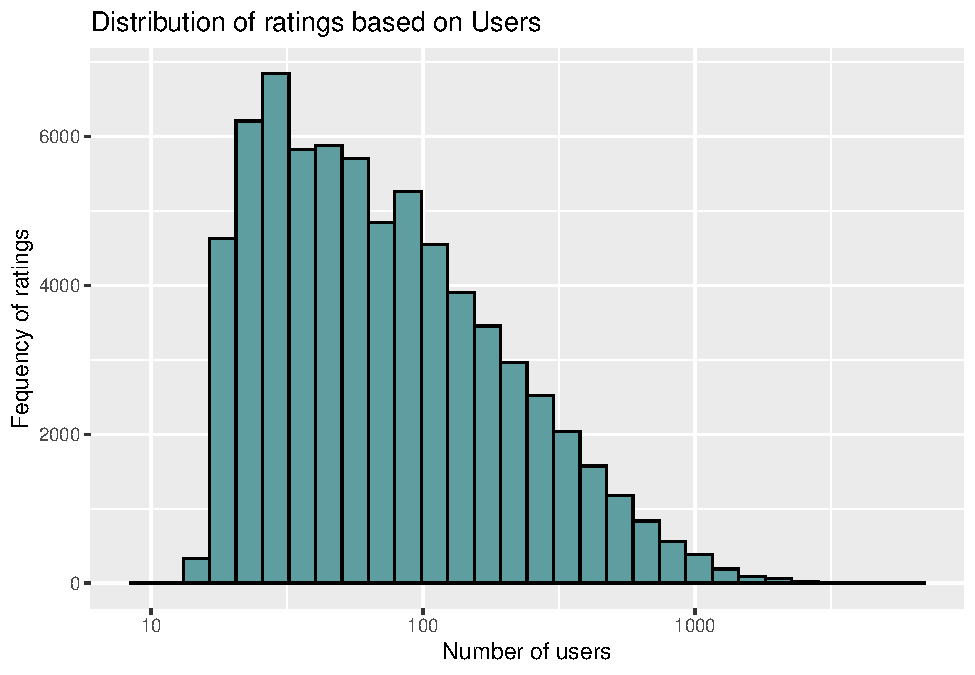
\includegraphics{Project_MovieLens_files/figure-latex/unnamed-chunk-9-1.pdf}

\subsection{Movies}
\label{sec:movies}

The dataset has around 10400 unique movies.

\begin{Shaded}
\begin{Highlighting}[]
\CommentTok{# Finding unique movies}
\NormalTok{edx }\OperatorTok\StringTok{ }\KeywordTok{summarize}\NormalTok{(}\DataTypeTok{movies =} \KeywordTok{n_distinct}\NormalTok{(title))}
\end{Highlighting}
\end{Shaded}

\begin{longtable}[]{@{}r@{}}
\toprule
movies\tabularnewline
\midrule
\endhead
10407\tabularnewline
\bottomrule
\end{longtable}

The release years for movies in \emph{edx} dataset range from 1915 to
2008. We can see an increase in the number of rated movies for the years
1980 to 1995. After 1995, the frequency of rated movies starts
decreasing---one of the possible reasons is that the dataset has not
included many movies for other years due to insufficient rating
information or the number of users providing the rating information
dropped.

\begin{Shaded}
\begin{Highlighting}[]
\KeywordTok{library}\NormalTok{(scales)}
\end{Highlighting}
\end{Shaded}

\begin{verbatim}
## 
## Attaching package: 'scales'
\end{verbatim}

\begin{verbatim}
## The following object is masked from 'package:purrr':
## 
##     discard
\end{verbatim}

\begin{verbatim}
## The following object is masked from 'package:readr':
## 
##     col_factor
\end{verbatim}

\begin{Shaded}
\begin{Highlighting}[]
\CommentTok{# Plotting frequency of rated moves over the years}
\CommentTok{# We use premiere years of movies as the range of years}
\NormalTok{edx }\OperatorTok
\StringTok{  }\KeywordTok{select}\NormalTok{(movieId, premiereYr) }\OperatorTok\StringTok{ }\CommentTok{# select columns we need}
\StringTok{  }\KeywordTok{group_by}\NormalTok{(premiereYr) }\OperatorTok\StringTok{ }\CommentTok{# group by year}
\StringTok{  }\KeywordTok{summarise}\NormalTok{(}\DataTypeTok{count =} \KeywordTok{n}\NormalTok{())  }\OperatorTok\StringTok{ }\CommentTok{# count movies per year}
\StringTok{  }\KeywordTok{arrange}\NormalTok{(premiereYr)}\OperatorTok
\StringTok{  }\KeywordTok{ggplot}\NormalTok{(}\KeywordTok{aes}\NormalTok{(}\DataTypeTok{x =}\NormalTok{ premiereYr, }\DataTypeTok{y =}\NormalTok{ count)) }\OperatorTok{+}
\StringTok{  }\KeywordTok{scale_y_log10}\NormalTok{() }\OperatorTok{+}
\StringTok{  }\KeywordTok{scale_y_continuous}\NormalTok{(}\DataTypeTok{breaks =} \KeywordTok{c}\NormalTok{(}\KeywordTok{seq}\NormalTok{(}\DecValTok{0}\NormalTok{, }\DecValTok{800000}\NormalTok{, }\DecValTok{100000}\NormalTok{)), }\DataTypeTok{labels=}\NormalTok{comma)}\OperatorTok{+}
\StringTok{  }\KeywordTok{labs}\NormalTok{(}\DataTypeTok{x=}\StringTok{"Movie Premiere Years"}\NormalTok{, }\DataTypeTok{y=}\StringTok{"Frequency of movies"}\NormalTok{) }\OperatorTok{+}
\StringTok{  }\KeywordTok{geom_point}\NormalTok{(}\DataTypeTok{color=}\StringTok{"cadetblue"}\NormalTok{) }\OperatorTok{+}
\StringTok{  }\KeywordTok{ggtitle}\NormalTok{(}\StringTok{"Distribution of rated movies with respect to premiere years"}\NormalTok{)}
\end{Highlighting}
\end{Shaded}

\begin{verbatim}
## Scale for 'y' is already present. Adding another scale for 'y', which
## will replace the existing scale.
\end{verbatim}

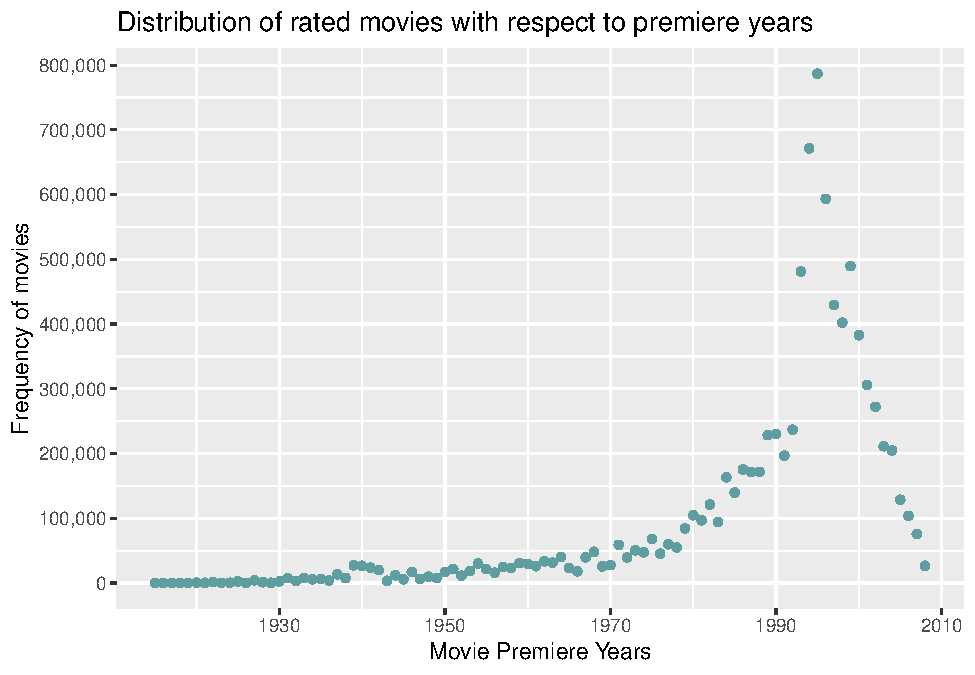
\includegraphics{Project_MovieLens_files/figure-latex/unnamed-chunk-11-1.pdf}
Most movies get a decent number of ratings from the users. Although some
movies have a less number of ratings. This indicates that movie
information can also be used as penalty term in our model (if required).

\begin{Shaded}
\begin{Highlighting}[]
\CommentTok{# Distribution or freqeuncy of ratings for all movies}
\NormalTok{edx }\OperatorTok\StringTok{ }\KeywordTok{group_by}\NormalTok{(movieId) }\OperatorTok\StringTok{ }\KeywordTok{summarize}\NormalTok{(}\DataTypeTok{n =} \KeywordTok{n}\NormalTok{()) }\OperatorTok
\StringTok{  }\KeywordTok{ggplot}\NormalTok{(}\KeywordTok{aes}\NormalTok{(n)) }\OperatorTok{+}\StringTok{ }\KeywordTok{geom_histogram}\NormalTok{(}\DataTypeTok{bins=}\DecValTok{30}\NormalTok{, }\DataTypeTok{fill =} \StringTok{'cadetblue'}\NormalTok{, }\DataTypeTok{color =} \StringTok{'black'}\NormalTok{) }\OperatorTok{+}
\StringTok{  }\KeywordTok{scale_x_log10}\NormalTok{() }\OperatorTok{+}
\StringTok{  }\KeywordTok{xlab}\NormalTok{(}\StringTok{"Number of movies"}\NormalTok{) }\OperatorTok{+}\StringTok{ }
\StringTok{  }\KeywordTok{ylab}\NormalTok{(}\StringTok{"Fequency of ratings"}\NormalTok{) }\OperatorTok{+}
\StringTok{  }\KeywordTok{ggtitle}\NormalTok{(}\StringTok{"Distribution of ratings per movie"}\NormalTok{)}
\end{Highlighting}
\end{Shaded}

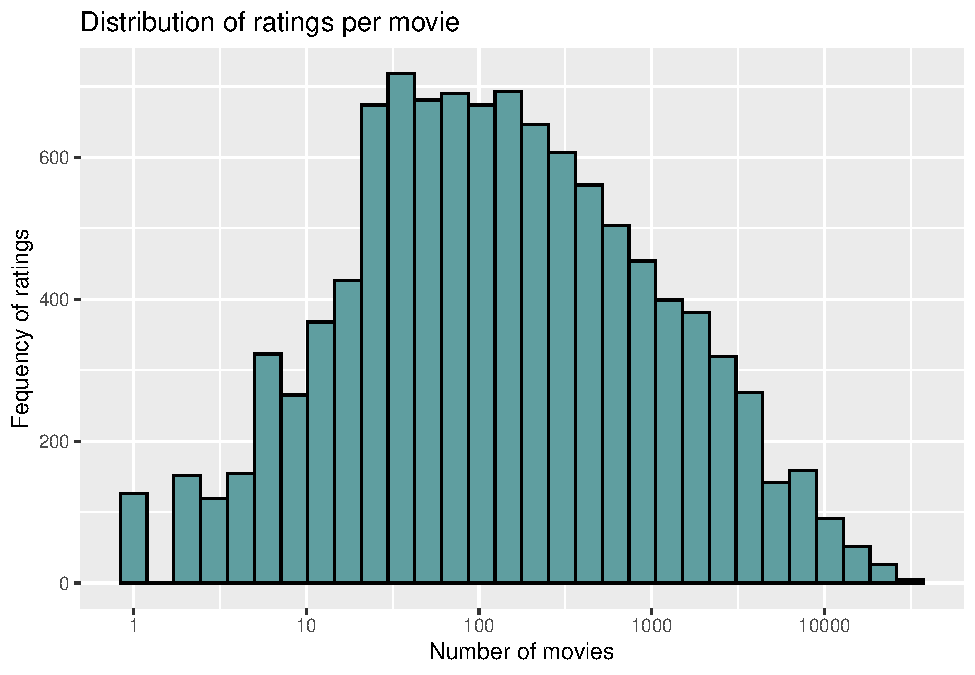
\includegraphics{Project_MovieLens_files/figure-latex/unnamed-chunk-12-1.pdf}

\subsection{Ratings}
\label{sec:ratings}

As we discussed in Section \label{sec:movies} that the release years of
movies in the dataset range from 1915 to 2008. The dataset also
indicates when users recorded the ratings for each movie. A close look
suggests that rating data covers a reasonable period from years 1995 to
2009 i.e., 14 years.

\begin{Shaded}
\begin{Highlighting}[]
\CommentTok{# Analysing when ratings data was added by users}
\NormalTok{years<-}\KeywordTok{format}\NormalTok{(edx}\OperatorTok{$}\NormalTok{timestamp, }\DataTypeTok{format=}\StringTok{"%Y"}\NormalTok{)}
\KeywordTok{sprintf}\NormalTok{(}\StringTok{"Rating year (minimum) =%s"}\NormalTok{, }\KeywordTok{min}\NormalTok{(years))}
\end{Highlighting}
\end{Shaded}

\begin{verbatim}
## [1] "Rating year (minimum) =1995"
\end{verbatim}

\begin{Shaded}
\begin{Highlighting}[]
\KeywordTok{sprintf}\NormalTok{(}\StringTok{"Rating year (maximu) =%s"}\NormalTok{, }\KeywordTok{max}\NormalTok{(years))}
\end{Highlighting}
\end{Shaded}

\begin{verbatim}
## [1] "Rating year (maximu) =2009"
\end{verbatim}

The movies can have either half-star or full-stars ratings. The
distribution indicates that most movies get full star ratings. We
observe that there is a tendency that users generally rate movies 3 or
4.

\begin{Shaded}
\begin{Highlighting}[]
\CommentTok{# Generating groups of data for half star and full star ratings}
\NormalTok{star_ratings_group <-}\StringTok{  }\KeywordTok{ifelse}\NormalTok{((edx}\OperatorTok{$}\NormalTok{rating }\OperatorTok{==}\StringTok{ }\DecValTok{1} \OperatorTok{|}\NormalTok{edx}\OperatorTok{$}\NormalTok{rating }\OperatorTok{==}\StringTok{ }\DecValTok{2} \OperatorTok{|}\StringTok{ }\NormalTok{edx}\OperatorTok{$}\NormalTok{rating }\OperatorTok{==}\StringTok{ }\DecValTok{3} \OperatorTok{|}\StringTok{ }
\StringTok{                  }\NormalTok{edx}\OperatorTok{$}\NormalTok{rating }\OperatorTok{==}\StringTok{ }\DecValTok{4} \OperatorTok{|}\StringTok{ }\NormalTok{edx}\OperatorTok{$}\NormalTok{rating }\OperatorTok{==}\StringTok{ }\DecValTok{5}\NormalTok{) ,}
                   \StringTok{"Full_star"}\NormalTok{, }
                   \StringTok{"Half_star"}\NormalTok{) }

\CommentTok{# Plotting the distribution of ratings in terms of half and full star}
\NormalTok{ratings_distribution <-}\StringTok{ }\KeywordTok{data.frame}\NormalTok{(edx}\OperatorTok{$}\NormalTok{rating, star_ratings_group)}
\KeywordTok{ggplot}\NormalTok{(ratings_distribution, }\KeywordTok{aes}\NormalTok{(}\DataTypeTok{x=}\NormalTok{ edx.rating, }\DataTypeTok{fill =}\NormalTok{ star_ratings_group)) }\OperatorTok{+}
\StringTok{  }\KeywordTok{geom_histogram}\NormalTok{( }\DataTypeTok{binwidth =} \FloatTok{0.2}\NormalTok{,}\DataTypeTok{color =} \StringTok{'black'}\NormalTok{) }\OperatorTok{+}
\StringTok{  }\KeywordTok{scale_x_discrete}\NormalTok{(}\DataTypeTok{limits =} \KeywordTok{c}\NormalTok{(}\KeywordTok{seq}\NormalTok{(}\FloatTok{0.5}\NormalTok{,}\DecValTok{5}\NormalTok{,}\FloatTok{0.5}\NormalTok{))) }\OperatorTok{+}
\StringTok{  }\KeywordTok{scale_y_continuous}\NormalTok{(}\DataTypeTok{breaks =} \KeywordTok{c}\NormalTok{(}\KeywordTok{seq}\NormalTok{(}\DecValTok{0}\NormalTok{, }\DecValTok{3000000}\NormalTok{, }\DecValTok{500000}\NormalTok{)))}\OperatorTok{+}
\StringTok{  }\KeywordTok{labs}\NormalTok{(}\DataTypeTok{x=}\StringTok{"Ratings"}\NormalTok{, }\DataTypeTok{y=}\StringTok{"Number of ratings"}\NormalTok{) }\OperatorTok{+}
\StringTok{  }\KeywordTok{ggtitle}\NormalTok{(}\StringTok{"Distribution of ratings"}\NormalTok{)}
\end{Highlighting}
\end{Shaded}

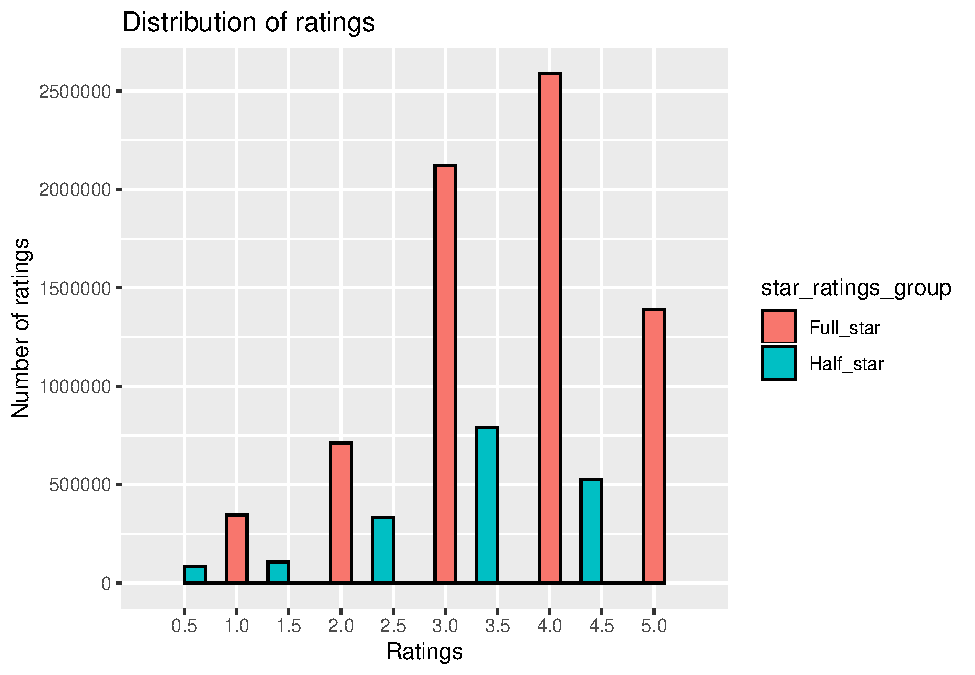
\includegraphics{Project_MovieLens_files/figure-latex/unnamed-chunk-14-1.pdf}

We now explore the top 10 and bottom 10 movies based on the total number
of ratings. Top 10 movies are well-known and many users rate them as
expected. Contrary, the bottom 10 movies appear to be obscure, and only
a few users rate them. Therefore, the predictions of future ratings for
such movies will be difficult. There are 125 movies in the dataset with
a single user rating. This information is critical because a low rating
numbers can result in overfitting for our model.

\begin{Shaded}
\begin{Highlighting}[]
\NormalTok{movies_count<-(edx }\OperatorTok\StringTok{ }\KeywordTok{group_by}\NormalTok{(title) }\OperatorTok\KeywordTok{summarize}\NormalTok{(}\DataTypeTok{count=}\KeywordTok{n}\NormalTok{()))}
\KeywordTok{sprintf}\NormalTok{(}\StringTok{"Movies with a single rating = %d"}\NormalTok{,}\KeywordTok{sum}\NormalTok{(movies_count}\OperatorTok{$}\NormalTok{count}\OperatorTok{==}\DecValTok{1}\NormalTok{))}
\end{Highlighting}
\end{Shaded}

\begin{verbatim}
## [1] "Movies with a single rating = 125"
\end{verbatim}

\begin{Shaded}
\begin{Highlighting}[]
\NormalTok{top_movies <-}\StringTok{ }\NormalTok{edx }\OperatorTok
\StringTok{  }\KeywordTok{group_by}\NormalTok{(title) }\OperatorTok
\StringTok{  }\KeywordTok{summarize}\NormalTok{(}\DataTypeTok{count=}\KeywordTok{n}\NormalTok{()) }\OperatorTok
\StringTok{  }\KeywordTok{top_n}\NormalTok{(}\DecValTok{10}\NormalTok{) }\OperatorTok
\StringTok{  }\KeywordTok{arrange}\NormalTok{(}\KeywordTok{desc}\NormalTok{(count))}
\end{Highlighting}
\end{Shaded}

\begin{verbatim}
## Selecting by count
\end{verbatim}

\begin{Shaded}
\begin{Highlighting}[]
\NormalTok{top_movies }\OperatorTok\StringTok{ }
\StringTok{  }\KeywordTok{ggplot}\NormalTok{(}\KeywordTok{aes}\NormalTok{(}\DataTypeTok{x=}\KeywordTok{reorder}\NormalTok{(title, count), }\DataTypeTok{y=}\NormalTok{count)) }\OperatorTok{+}
\StringTok{  }\KeywordTok{geom_bar}\NormalTok{(}\DataTypeTok{stat=}\StringTok{'identity'}\NormalTok{, }\DataTypeTok{fill=}\StringTok{"cadetblue"}\NormalTok{) }\OperatorTok{+}\StringTok{ }\KeywordTok{coord_flip}\NormalTok{(}\DataTypeTok{y=}\KeywordTok{c}\NormalTok{(}\DecValTok{0}\NormalTok{, }\DecValTok{40000}\NormalTok{)) }\OperatorTok{+}
\StringTok{  }\KeywordTok{labs}\NormalTok{(}\DataTypeTok{x=}\StringTok{""}\NormalTok{, }\DataTypeTok{y=}\StringTok{"Number of ratings"}\NormalTok{) }\OperatorTok{+}
\StringTok{  }\KeywordTok{geom_text}\NormalTok{(}\KeywordTok{aes}\NormalTok{(}\DataTypeTok{label=}\NormalTok{ count), }\DataTypeTok{hjust=}\OperatorTok{-}\FloatTok{0.1}\NormalTok{, }\DataTypeTok{size=}\DecValTok{3}\NormalTok{) }\OperatorTok{+}
\StringTok{  }\KeywordTok{labs}\NormalTok{(}\DataTypeTok{title=}\StringTok{"Top 10 movies titles based on number of ratings"}\NormalTok{ )}
\end{Highlighting}
\end{Shaded}

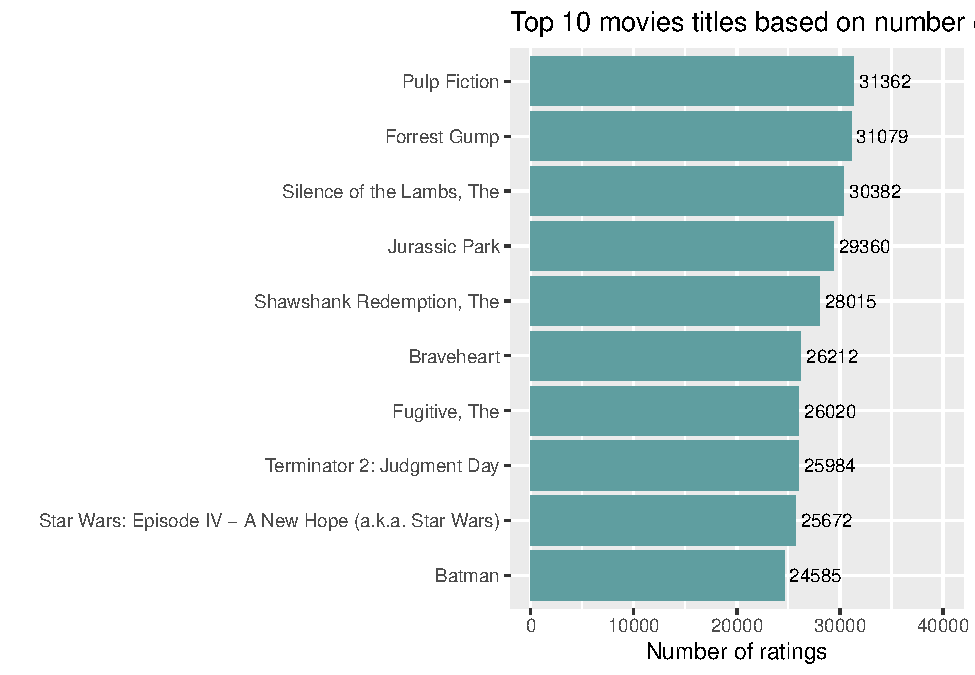
\includegraphics{Project_MovieLens_files/figure-latex/unnamed-chunk-16-1.pdf}

\begin{Shaded}
\begin{Highlighting}[]
\NormalTok{bottom_movies <-}\StringTok{ }\NormalTok{edx }\OperatorTok
\StringTok{  }\KeywordTok{group_by}\NormalTok{(title) }\OperatorTok
\StringTok{  }\KeywordTok{summarize}\NormalTok{(}\DataTypeTok{count=}\KeywordTok{n}\NormalTok{()) }\OperatorTok
\StringTok{  }\KeywordTok{arrange}\NormalTok{(}\KeywordTok{desc}\NormalTok{(count))}

\NormalTok{bottom_movies }\OperatorTok\StringTok{ }\KeywordTok{tail}\NormalTok{(}\DecValTok{10}\NormalTok{) }\OperatorTok
\StringTok{  }\KeywordTok{ggplot}\NormalTok{(}\KeywordTok{aes}\NormalTok{(}\DataTypeTok{x=}\KeywordTok{reorder}\NormalTok{(title, count), }\DataTypeTok{y=}\NormalTok{count)) }\OperatorTok{+}
\StringTok{  }\KeywordTok{geom_bar}\NormalTok{(}\DataTypeTok{stat=}\StringTok{'identity'}\NormalTok{, }\DataTypeTok{fill=}\StringTok{"cadetblue"}\NormalTok{) }\OperatorTok{+}\StringTok{ }\KeywordTok{coord_flip}\NormalTok{(}\DataTypeTok{y=}\KeywordTok{c}\NormalTok{(}\DecValTok{0}\NormalTok{, }\DecValTok{100}\NormalTok{)) }\OperatorTok{+}
\StringTok{  }\KeywordTok{labs}\NormalTok{(}\DataTypeTok{x=}\StringTok{""}\NormalTok{, }\DataTypeTok{y=}\StringTok{"Number of ratings"}\NormalTok{) }\OperatorTok{+}
\StringTok{  }\KeywordTok{geom_text}\NormalTok{(}\KeywordTok{aes}\NormalTok{(}\DataTypeTok{label=}\NormalTok{ count), }\DataTypeTok{hjust=}\OperatorTok{-}\FloatTok{0.1}\NormalTok{, }\DataTypeTok{size=}\DecValTok{3}\NormalTok{) }\OperatorTok{+}
\StringTok{  }\KeywordTok{labs}\NormalTok{(}\DataTypeTok{title=}\StringTok{"Bottom 10 movies based on number of ratings"}\NormalTok{)}
\end{Highlighting}
\end{Shaded}

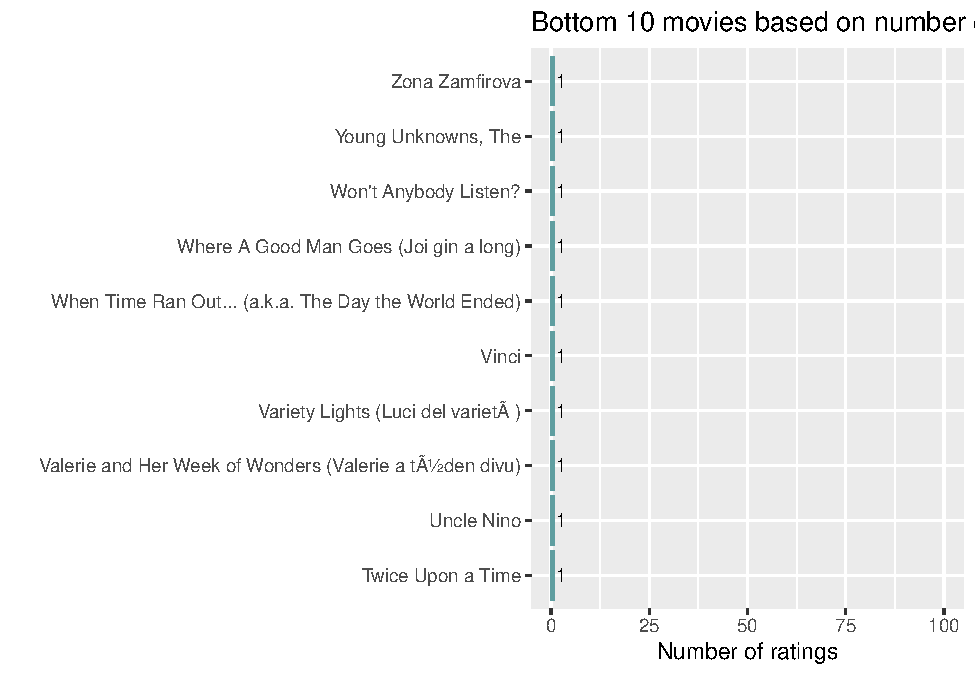
\includegraphics{Project_MovieLens_files/figure-latex/unnamed-chunk-17-1.pdf}

\subsection{Generes}
\label{sec:generes}

Each movie can have more than one genre. A close analysis indicates that
most movies in the dataset belong to \texttt{Comedy"\ and}Drama" genres.
A very few movies belong to the ``fantasy" genre. Therefore, we can also
use this feature as a penalty term in our model (if required). Moreover,
there are some movies with untitled genres. We can remove them if
needed.

\begin{Shaded}
\begin{Highlighting}[]
\CommentTok{# Extracting all unique combination of genres}
\NormalTok{unique_genres_combination<-edx}\OperatorTok\StringTok{ }\KeywordTok{group_by}\NormalTok{(genres)}\OperatorTok\KeywordTok{summarize}\NormalTok{(}\DataTypeTok{count =} \KeywordTok{n}\NormalTok{())}

\CommentTok{# Extract all possible genres (which exist in the dataset)}
\NormalTok{movie_genres <-}\StringTok{ }\KeywordTok{unique}\NormalTok{(}\KeywordTok{unlist}\NormalTok{(}\KeywordTok{strsplit}\NormalTok{(}\KeywordTok{unique}\NormalTok{(edx}\OperatorTok{$}\NormalTok{genres), }\DataTypeTok{split=}\StringTok{'|'}\NormalTok{, }\DataTypeTok{fixed=}\OtherTok{TRUE}\NormalTok{)))}
\NormalTok{movie_genres <-}\StringTok{ }\KeywordTok{as.data.frame}\NormalTok{(movie_genres)}
\NormalTok{movie_genres<-movie_genres }\OperatorTok\StringTok{ }\KeywordTok{add_column}\NormalTok{(}\DataTypeTok{count =} \DecValTok{0}\NormalTok{)}

\CommentTok{# Looping through to find the freqeucny or distribution of each genre}
\ControlFlowTok{for}\NormalTok{(i }\ControlFlowTok{in} \DecValTok{1}\OperatorTok{:}\KeywordTok{dim}\NormalTok{(movie_genres)[}\DecValTok{1}\NormalTok{]) \{}
  \ControlFlowTok{for}\NormalTok{(j }\ControlFlowTok{in} \DecValTok{1}\OperatorTok{:}\KeywordTok{dim}\NormalTok{(unique_genres_combination)[}\DecValTok{1}\NormalTok{])}
\NormalTok{  \{}
\NormalTok{    match =}\StringTok{ }\KeywordTok{as.character}\NormalTok{(unique_genres_combination[j,}\DecValTok{1}\NormalTok{])}
\NormalTok{    count =}\StringTok{ }\KeywordTok{as.numeric}\NormalTok{(unique_genres_combination[j,}\DecValTok{2}\NormalTok{])}
    \CommentTok{# See if genre category exists in the combination}
    \ControlFlowTok{if}\NormalTok{ (}\KeywordTok{str_contains}\NormalTok{(movie_genres[i,}\DecValTok{1}\NormalTok{],match))}
\NormalTok{    \{}
\NormalTok{      movie_genres[i,}\DecValTok{2}\NormalTok{]<-movie_genres[i,}\DecValTok{2}\NormalTok{]}\OperatorTok{+}\NormalTok{count}
\NormalTok{    \}}
\NormalTok{  \}}
\NormalTok{\}}

\CommentTok{# Plot distrobution of movie genres }
\NormalTok{movie_genres}\OperatorTok
\StringTok{  }\KeywordTok{ggplot}\NormalTok{(}\KeywordTok{aes}\NormalTok{(}\DataTypeTok{x=}\KeywordTok{reorder}\NormalTok{(movie_genres, count), }\DataTypeTok{y=}\NormalTok{count)) }\OperatorTok{+}
\StringTok{  }\KeywordTok{geom_bar}\NormalTok{(}\DataTypeTok{stat=}\StringTok{'identity'}\NormalTok{, }\DataTypeTok{fill=}\StringTok{"cadetblue"}\NormalTok{) }\OperatorTok{+}\StringTok{ }\KeywordTok{coord_flip}\NormalTok{(}\DataTypeTok{y=}\KeywordTok{c}\NormalTok{(}\DecValTok{0}\NormalTok{, }\DecValTok{900000}\NormalTok{)) }\OperatorTok{+}
\StringTok{  }\KeywordTok{labs}\NormalTok{(}\DataTypeTok{x=}\StringTok{"Count"}\NormalTok{, }\DataTypeTok{y=}\StringTok{"Movie genres"}\NormalTok{) }\OperatorTok{+}
\StringTok{  }\KeywordTok{geom_text}\NormalTok{(}\KeywordTok{aes}\NormalTok{(}\DataTypeTok{label=}\NormalTok{ count), }\DataTypeTok{hjust=}\OperatorTok{-}\FloatTok{0.1}\NormalTok{, }\DataTypeTok{size=}\DecValTok{3}\NormalTok{) }\OperatorTok{+}
\StringTok{  }\KeywordTok{labs}\NormalTok{(}\DataTypeTok{title=}\StringTok{"Distribution of movies based on genre"}\NormalTok{ )}
\end{Highlighting}
\end{Shaded}

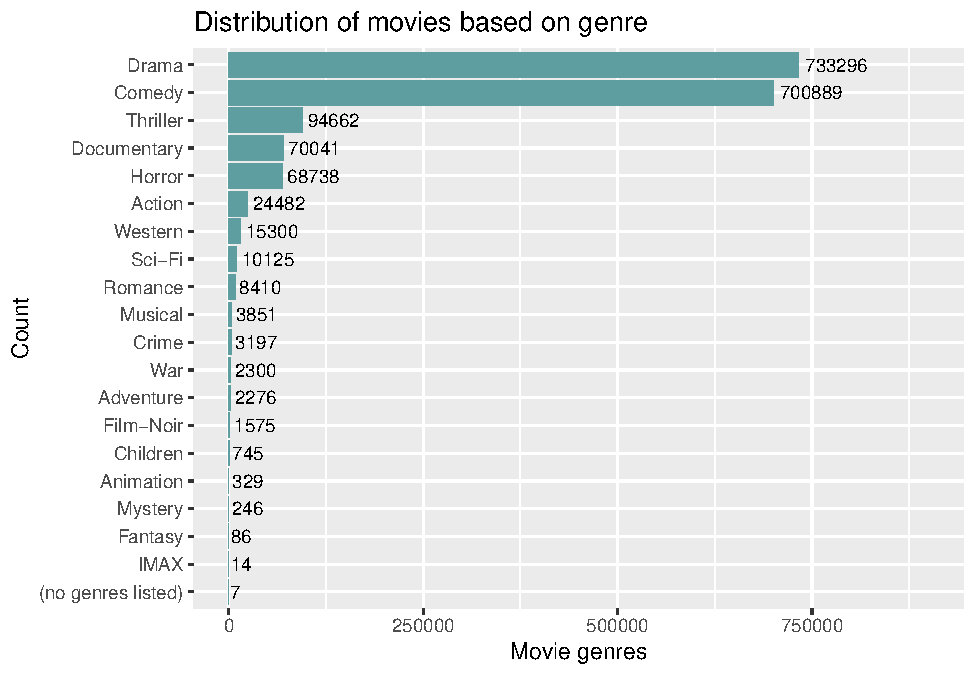
\includegraphics{Project_MovieLens_files/figure-latex/unnamed-chunk-18-1.pdf}

\subsection{Premier Year}
\label{sec:pyear}

We analyse the rating trends of users over the years. Interestingly, we
find out that mean ratings have dropped over the years. This indicates
that users are not rating more movies in recent years.

\begin{Shaded}
\begin{Highlighting}[]
\NormalTok{edx }\OperatorTok\StringTok{ }\KeywordTok{group_by}\NormalTok{(premiereYr) }\OperatorTok
\StringTok{  }\KeywordTok{summarize}\NormalTok{(}\DataTypeTok{rating =} \KeywordTok{mean}\NormalTok{(rating)) }\OperatorTok
\StringTok{  }\KeywordTok{ggplot}\NormalTok{(}\KeywordTok{aes}\NormalTok{(premiereYr, rating)) }\OperatorTok{+}
\StringTok{  }\KeywordTok{geom_point}\NormalTok{() }\OperatorTok{+}
\StringTok{  }\KeywordTok{labs}\NormalTok{(}\DataTypeTok{x=}\StringTok{"Years"}\NormalTok{, }\DataTypeTok{y=}\StringTok{"Mean Rating"}\NormalTok{)}\OperatorTok{+}
\StringTok{  }\KeywordTok{geom_smooth}\NormalTok{(}\DataTypeTok{alpha=}\FloatTok{0.5}\NormalTok{, }\DataTypeTok{color=}\StringTok{'cadetblue'}\NormalTok{,}\DataTypeTok{method =}\NormalTok{ lm,}\DataTypeTok{formula =}\NormalTok{ y }\OperatorTok{~}\StringTok{ }\NormalTok{splines}\OperatorTok{::}\KeywordTok{bs}\NormalTok{(x, }\DecValTok{3}\NormalTok{))}
\end{Highlighting}
\end{Shaded}

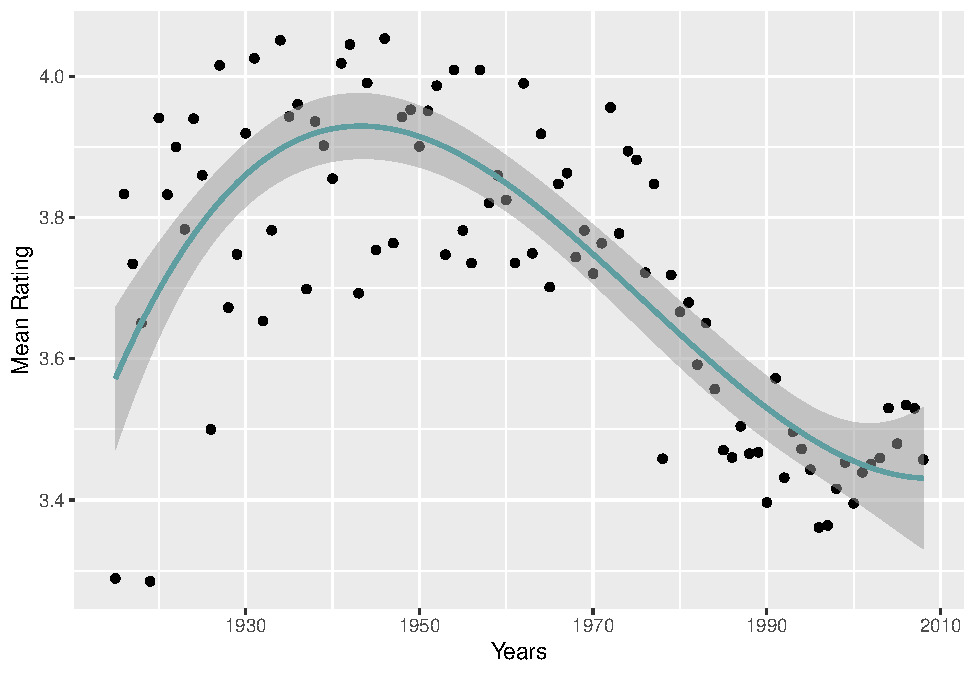
\includegraphics{Project_MovieLens_files/figure-latex/unnamed-chunk-19-1.pdf}

\section{Methods}
\label{sec:methods}

We will use RMSE to estimate the quality of our model. We define
\(y_{u,i}\) as the rating for the movie \(i\) and donate prediction by
\(\hat{y}_{u,i}\) as shown below:

\begin{equation}
\label{eq:rmsefinal}
RMSE = \sqrt{\frac{1}{N}\displaystyle\sum_{i=1}^{n} (\hat{y}_{u,i}-y_{u,i})^{2}}
\end{equation}For our problem, as the rating for movie

Where N is the number of user/movie combinations. Using Equation
\ref{eq:rmsefinal}, we write the following function to compute the RMSE:

\begin{Shaded}
\begin{Highlighting}[]
\NormalTok{RMSE <-}\StringTok{ }\ControlFlowTok{function}\NormalTok{(true_ratings, predicted_ratings)\{}
  \KeywordTok{sqrt}\NormalTok{(}\KeywordTok{mean}\NormalTok{((true_ratings }\OperatorTok{-}\StringTok{ }\NormalTok{predicted_ratings)}\OperatorTok{^}\DecValTok{2}\NormalTok{))}
\NormalTok{\}}
\end{Highlighting}
\end{Shaded}

The lower RMSE better is the model. The evaluation criteria for this
project is that the RMSE of the proposed model should be less than
0.8649.

\begin{Shaded}
\begin{Highlighting}[]
\CommentTok{#Initiate RMSE results to compare various models}
\NormalTok{rmse_results <-}\StringTok{ }\KeywordTok{data_frame}\NormalTok{(}\DataTypeTok{method =} \StringTok{"Target RSME"}\NormalTok{, }\DataTypeTok{RMSE =} \FloatTok{0.86490}\NormalTok{)}
\end{Highlighting}
\end{Shaded}

\begin{verbatim}
## Warning: `data_frame()` is deprecated, use `tibble()`.
## This warning is displayed once per session.
\end{verbatim}

\begin{Shaded}
\begin{Highlighting}[]
\NormalTok{rmse_results}
\end{Highlighting}
\end{Shaded}

\begin{longtable}[]{@{}lr@{}}
\toprule
method & RMSE\tabularnewline
\midrule
\endhead
Target RSME & 0.8649\tabularnewline
\bottomrule
\end{longtable}

\subsection{Average Movie Rating Model}
\label{sec:am}

We start with the simplest model by predicting the same ratings for all
movies regardless of users or frequency of ratings. So, we compute the
dataset's mean rating:

\begin{equation}
Y_{u, i} = \mu + \epsilon_{u, i}
\end{equation}

Where \(\epsilon_{u,i}\) is the independent error sample from the same
distribution centered at 0 and \(\mu\) the true rating for all movies.
This model uses the assumption that differences in movie ratings are
explainable by random variation alone. The expected value (\(\mu\)) of
the data is around 3.5. We make predictions using \(\mu\), and the
resulting RMSE of the model is 1.06 on validation data.

\begin{Shaded}
\begin{Highlighting}[]
\CommentTok{# Calculating mean of ratings}
\NormalTok{mean_rating <-}\StringTok{ }\KeywordTok{mean}\NormalTok{(edx}\OperatorTok{$}\NormalTok{rating)}
\NormalTok{mean_rating}
\end{Highlighting}
\end{Shaded}

\begin{verbatim}
## [1] 3.512465
\end{verbatim}

\begin{Shaded}
\begin{Highlighting}[]
\CommentTok{# Making predictions using mean rating}
\NormalTok{mean_model_rmse <-}\StringTok{ }\KeywordTok{RMSE}\NormalTok{(validation}\OperatorTok{$}\NormalTok{rating, mean_rating)}
\NormalTok{rmse_results <-}\StringTok{ }\KeywordTok{bind_rows}\NormalTok{(rmse_results,}
                          \KeywordTok{data_frame}\NormalTok{(}\DataTypeTok{method=}\StringTok{"Average Rating Model"}\NormalTok{,  }
                                     \DataTypeTok{RMSE =}\NormalTok{ mean_model_rmse ))}
\NormalTok{rmse_results}
\end{Highlighting}
\end{Shaded}

\begin{longtable}[]{@{}lr@{}}
\toprule
method & RMSE\tabularnewline
\midrule
\endhead
Target RSME & 0.864900\tabularnewline
Average Rating Model & 1.061202\tabularnewline
\bottomrule
\end{longtable}

\subsection{Model with movie effect}
\label{sec:mem}

The RMSE of our previous model is very high compared to the target RMSE.
To improve the RMSE of our model, we have to include extra parameters in
our model. We recall from Section \ref{sec:dataanalsyis} that different
movies are rated differently. The popular movies are rated much higher
than unpopular movies. We modify the previous model by adding the term
`\(b_{i}\)" to represent the average ranking for movie \(i\) as follows:

\begin{equation}
Y_{u, i} = \mu +b_{i}+ \epsilon_{u, i}
\end{equation}

The least-squares estimate \(b_{i}\) is just the average of
\(Y_{u,i} - \mu\) for each movie \(i\). We can compute it as follows:

\begin{Shaded}
\begin{Highlighting}[]
\CommentTok{# Computing average ranking for movie "i"}
\NormalTok{movie_averages <-}\StringTok{ }\NormalTok{edx }\OperatorTok
\StringTok{  }\KeywordTok{group_by}\NormalTok{(movieId) }\OperatorTok
\StringTok{  }\KeywordTok{summarize}\NormalTok{(}\DataTypeTok{b_i =} \KeywordTok{mean}\NormalTok{(rating }\OperatorTok{-}\StringTok{ }\NormalTok{mean_rating))}
\end{Highlighting}
\end{Shaded}

The histogram of average rankings for movies is not symmetric and is
skewed to the left (towards negative rating effect). This is known as
the penalty term movie effect and supports the idea of using it in our
model.

\begin{Shaded}
\begin{Highlighting}[]
\CommentTok{# Plotting average ranking estimates for movies}
\NormalTok{movie_averages}\OperatorTok
\StringTok{  }\KeywordTok{ggplot}\NormalTok{(}\KeywordTok{aes}\NormalTok{(b_i)) }\OperatorTok{+}
\StringTok{  }\KeywordTok{labs}\NormalTok{(}\DataTypeTok{x=}\StringTok{"b_i"}\NormalTok{, }\DataTypeTok{y=}\StringTok{"Count"}\NormalTok{)}\OperatorTok{+}
\StringTok{  }\KeywordTok{geom_histogram}\NormalTok{(}\DataTypeTok{bins =} \DecValTok{30}\NormalTok{, }\DataTypeTok{color =} \StringTok{"black"}\NormalTok{)}
\end{Highlighting}
\end{Shaded}

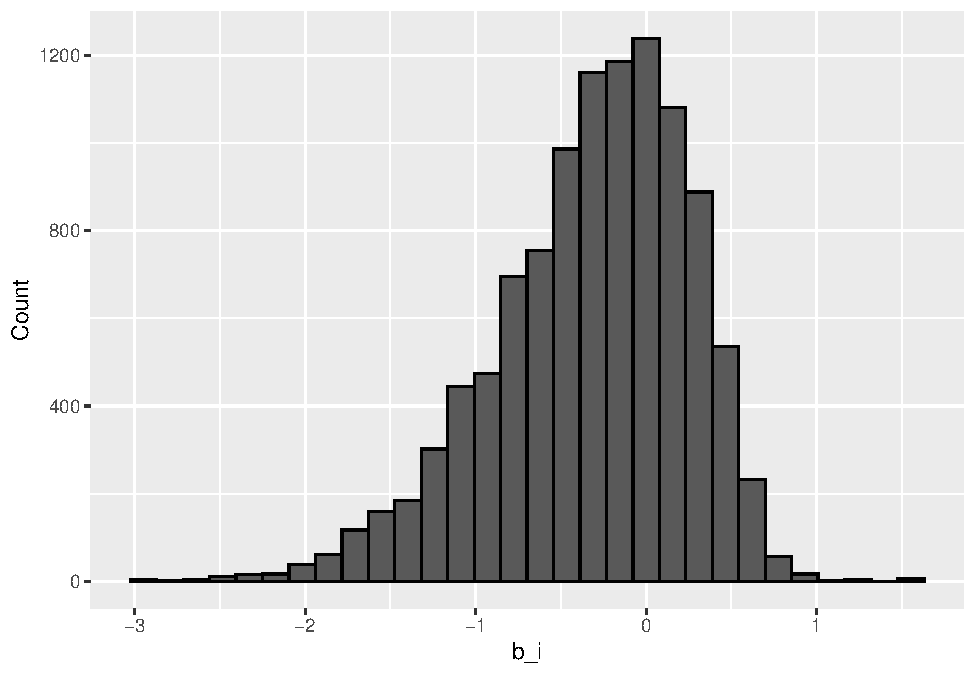
\includegraphics{Project_MovieLens_files/figure-latex/unnamed-chunk-24-1.pdf}
If one movie is on average rated better than the average rating of all
movies \(\mu\), then we predict that it will be rated higher than
\(\mu\) by \(b_{i}\).By including the movie effect, the RMSE of the
model improves to 0.9439 on validation data.

\begin{Shaded}
\begin{Highlighting}[]
\CommentTok{# Making predictions using new model}
\NormalTok{predicted_ratings <-}\StringTok{ }\NormalTok{mean_rating }\OperatorTok{+}\StringTok{  }\NormalTok{validation }\OperatorTok
\StringTok{  }\KeywordTok{left_join}\NormalTok{(movie_averages, }\DataTypeTok{by=}\StringTok{'movieId'}\NormalTok{) }\OperatorTok
\StringTok{  }\KeywordTok{pull}\NormalTok{(b_i)}

\CommentTok{# Calculating RMSE}
\NormalTok{model_movie_effects_rmse <-}\StringTok{ }\KeywordTok{RMSE}\NormalTok{(predicted_ratings, validation}\OperatorTok{$}\NormalTok{rating)}

\CommentTok{# Appending results to RMSE table}
\NormalTok{rmse_results <-}\StringTok{ }\KeywordTok{bind_rows}\NormalTok{(rmse_results,}
                          \KeywordTok{data_frame}\NormalTok{(}\DataTypeTok{method=}\StringTok{"Movie effect model"}\NormalTok{,  }
                                     \DataTypeTok{RMSE =}\NormalTok{ model_movie_effects_rmse ))}
\NormalTok{rmse_results}
\end{Highlighting}
\end{Shaded}

\begin{longtable}[]{@{}lr@{}}
\toprule
method & RMSE\tabularnewline
\midrule
\endhead
Target RSME & 0.8649000\tabularnewline
Average Rating Model & 1.0612018\tabularnewline
Movie effect model & 0.9439087\tabularnewline
\bottomrule
\end{longtable}

\section{Model with user effects}
\label{sec:uer}

We know that some users are more active in rating than others. We
compute the average rating for user \(u\), who have rated over 100
movies. We notice a substantial variability across users. Some users are
very cranky (like few movies), while others love every movie. Therefore,
we can further improve our previous model by adding user-specific effect
(\(b_{u}\)):

\begin{equation}
Y_{u, i} = \mu + b_{i} + b_{u} + \epsilon_{u, i}
\end{equation}

\begin{Shaded}
\begin{Highlighting}[]
\CommentTok{# Calculating average rating for user u}
\NormalTok{user_averages <-}\StringTok{ }\NormalTok{edx }\OperatorTok
\StringTok{  }\KeywordTok{left_join}\NormalTok{(movie_averages, }\DataTypeTok{by=}\StringTok{'movieId'}\NormalTok{) }\OperatorTok
\StringTok{  }\KeywordTok{group_by}\NormalTok{(userId) }\OperatorTok
\StringTok{  }\KeywordTok{summarize}\NormalTok{(}\DataTypeTok{b_u =} \KeywordTok{mean}\NormalTok{(rating }\OperatorTok{-}\StringTok{ }\NormalTok{mean_rating }\OperatorTok{-}\StringTok{ }\NormalTok{b_i))}

\CommentTok{# Plotting average rating for users}
\NormalTok{user_averages }\OperatorTok
\StringTok{  }\KeywordTok{ggplot}\NormalTok{(}\KeywordTok{aes}\NormalTok{(b_u)) }\OperatorTok{+}
\StringTok{  }\KeywordTok{labs}\NormalTok{(}\DataTypeTok{x=}\StringTok{"u_i"}\NormalTok{, }\DataTypeTok{y=}\StringTok{"Count"}\NormalTok{)}\OperatorTok{+}
\StringTok{  }\KeywordTok{geom_histogram}\NormalTok{(}\DataTypeTok{bins =} \DecValTok{10}\NormalTok{, }\DataTypeTok{color =} \StringTok{"black"}\NormalTok{)}
\end{Highlighting}
\end{Shaded}

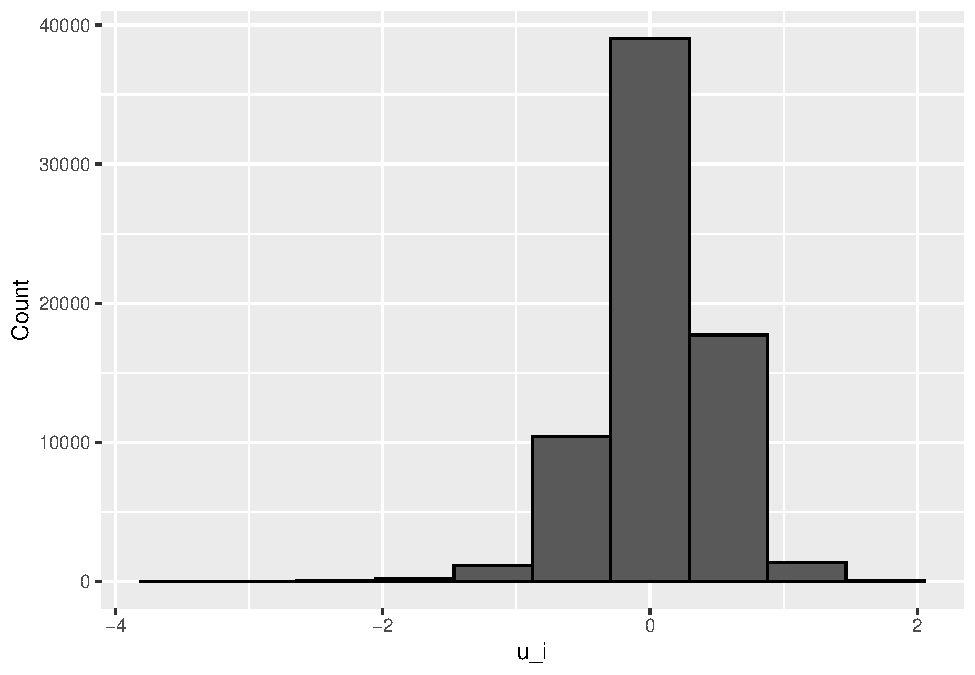
\includegraphics{Project_MovieLens_files/figure-latex/unnamed-chunk-26-1.pdf}

If a cranky user (negative \(b_{u}\)) rates a great movie (positive
\(b_{i}\)), the effects counter each other. And we may be able to
correctly predict that this user gave this great movie a 3 rather than a
5. By using the new model for prediction on the validation dataset, the
RMSE improves to 0.8653.

\begin{Shaded}
\begin{Highlighting}[]
\CommentTok{# Making predictions using new model}
\NormalTok{predicted_ratings <-}\StringTok{ }\NormalTok{validation}\OperatorTok
\StringTok{  }\KeywordTok{left_join}\NormalTok{(movie_averages, }\DataTypeTok{by=}\StringTok{'movieId'}\NormalTok{) }\OperatorTok
\StringTok{  }\KeywordTok{left_join}\NormalTok{(user_averages, }\DataTypeTok{by=}\StringTok{'userId'}\NormalTok{) }\OperatorTok
\StringTok{  }\KeywordTok{mutate}\NormalTok{(}\DataTypeTok{pred =}\NormalTok{ mean_rating }\OperatorTok{+}\StringTok{ }\NormalTok{b_i }\OperatorTok{+}\StringTok{ }\NormalTok{b_u) }\OperatorTok
\StringTok{  }\KeywordTok{pull}\NormalTok{(pred)}

\CommentTok{# Calculating RMSE on validation dataset}
\NormalTok{model_user_effect_rmse <-}\StringTok{ }\KeywordTok{RMSE}\NormalTok{(predicted_ratings, validation}\OperatorTok{$}\NormalTok{rating)}

\CommentTok{# Appending results to RMSE table}
\NormalTok{rmse_results <-}\StringTok{ }\KeywordTok{bind_rows}\NormalTok{(rmse_results,}
                          \KeywordTok{data_frame}\NormalTok{(}\DataTypeTok{method=}\StringTok{"Movie and user effect model"}\NormalTok{,  }
                                     \DataTypeTok{RMSE =}\NormalTok{ model_user_effect_rmse))}
\NormalTok{rmse_results}
\end{Highlighting}
\end{Shaded}

\begin{longtable}[]{@{}lr@{}}
\toprule
method & RMSE\tabularnewline
\midrule
\endhead
Target RSME & 0.8649000\tabularnewline
Average Rating Model & 1.0612018\tabularnewline
Movie effect model & 0.9439087\tabularnewline
Movie and user effect model & 0.8653488\tabularnewline
\bottomrule
\end{longtable}

\subsection{Regularization using movie and user effects}
\subsection{sec:reg}

We made mistakes on our first model when we used the effect of movies
only.

\begin{enumerate}
\item There are users who have rated very few movies (less than 30 movies). On the other hand, 
\item Some movies are rated very few times (as low as 1). 
\end{enumerate}

These are noisy estimates that result in overfitting of the model.
Because the model tries hard to fit the noisy estimates, such large
errors are likely to increase the RMSE and affect the predictions.

To solve this problem, we use Regularization. The Regularization permits
to penalize large estimates that come from small sample sizes. The
general idea of penalized regression is to control the total variability
of the movie effects. Instead of minimizing the least squares equation,
we minimize an equation that adds a penalty that gets larger when many
\(b_{i}\) are large:

\begin{equation}
\frac{1}{N} \sum_{u,i} \left(y_{u,i} - \mu - b_i\right)^2 + \lambda \sum_{i} b_i^2
\end{equation}

The values of \(b_{i}\) that minimise the above equation are :

\begin{equation}
\hat{b}_i(\lambda) = \frac{1}{\lambda + n_i} \sum_{u=1}^{n_i} \left(Y_{u,i} - \hat{\mu}\right)
\end{equation}

Where \(n_{i}\) is the number of ratings made for movie \(i\). This
approach will have our desired effect because when our sample size \(n\)
is very large, then we will get a stable estimate, and the penalty
\(\lambda\) is effectively ignored. However, with a small sample size,
the estimate \(\hat{b}_i(\lambda)\) will shrink towards zero. We can use
regularization to estimate of user effects as well as shown below:

\begin{equation}
\frac{1}{N} \sum_{u,i} \left(y_{u,i} - \mu - b_i - b_u \right)^2 + 
\lambda \left(\sum_{i} b_i^2 + \sum_{u} b_u^2\right)
\end{equation}

We can see that it is important to find an optimal value of our tuning
parameter \(\lamda\) which will minimise the value of RMSE. We find
optimal \(\lambda\) giving us the best RMSE score as follow.

\begin{Shaded}
\begin{Highlighting}[]
\CommentTok{# Possible Lambda values}
\NormalTok{lambdas <-}\StringTok{ }\KeywordTok{seq}\NormalTok{(}\DecValTok{0}\NormalTok{, }\DecValTok{10}\NormalTok{, }\FloatTok{0.25}\NormalTok{)}

\CommentTok{# Calculating mean of model}
\NormalTok{mean_rating <-}\StringTok{ }\KeywordTok{mean}\NormalTok{(edx}\OperatorTok{$}\NormalTok{rating)}
\NormalTok{rmses <-}\StringTok{ }\KeywordTok{sapply}\NormalTok{(lambdas, }\ControlFlowTok{function}\NormalTok{(l)\{}
  \CommentTok{# Penalised movie effect}
\NormalTok{  b_i <-}\StringTok{ }\NormalTok{edx }\OperatorTok\StringTok{ }
\StringTok{    }\KeywordTok{group_by}\NormalTok{(movieId) }\OperatorTok
\StringTok{    }\KeywordTok{summarize}\NormalTok{(}\DataTypeTok{b_i =} \KeywordTok{sum}\NormalTok{(rating }\OperatorTok{-}\StringTok{ }\NormalTok{mean_rating)}\OperatorTok{/}\NormalTok{(}\KeywordTok{n}\NormalTok{()}\OperatorTok{+}\NormalTok{l))}
  \CommentTok{# Penalised user effect}
\NormalTok{  b_u <-}\StringTok{ }\NormalTok{edx }\OperatorTok\StringTok{ }
\StringTok{    }\KeywordTok{left_join}\NormalTok{(b_i, }\DataTypeTok{by=}\StringTok{"movieId"}\NormalTok{) }\OperatorTok
\StringTok{    }\KeywordTok{group_by}\NormalTok{(userId) }\OperatorTok
\StringTok{    }\KeywordTok{summarize}\NormalTok{(}\DataTypeTok{b_u =} \KeywordTok{sum}\NormalTok{(rating }\OperatorTok{-}\StringTok{ }\NormalTok{b_i }\OperatorTok{-}\StringTok{ }\NormalTok{mean_rating)}\OperatorTok{/}\NormalTok{(}\KeywordTok{n}\NormalTok{()}\OperatorTok{+}\NormalTok{l))}
  \CommentTok{# Predicting new ratings}
\NormalTok{  predicted_ratings <-}\StringTok{ }
\StringTok{    }\NormalTok{validation }\OperatorTok\StringTok{ }
\StringTok{    }\KeywordTok{left_join}\NormalTok{(b_i, }\DataTypeTok{by =} \StringTok{"movieId"}\NormalTok{) }\OperatorTok
\StringTok{    }\KeywordTok{left_join}\NormalTok{(b_u, }\DataTypeTok{by =} \StringTok{"userId"}\NormalTok{) }\OperatorTok
\StringTok{    }\KeywordTok{mutate}\NormalTok{(}\DataTypeTok{pred =}\NormalTok{ mean_rating }\OperatorTok{+}\StringTok{ }\NormalTok{b_i }\OperatorTok{+}\StringTok{ }\NormalTok{b_u) }\OperatorTok
\StringTok{    }\KeywordTok{pull}\NormalTok{(pred)}
  
  \KeywordTok{return}\NormalTok{(}\KeywordTok{RMSE}\NormalTok{(predicted_ratings, validation}\OperatorTok{$}\NormalTok{rating))}
\NormalTok{\})}
\end{Highlighting}
\end{Shaded}

The optimal lambda value is 5.25, which gives us an RMSE of 0.864817.

\begin{Shaded}
\begin{Highlighting}[]
\NormalTok{lambda <-}\StringTok{ }\NormalTok{lambdas[}\KeywordTok{which.min}\NormalTok{(rmses)]}
\KeywordTok{qplot}\NormalTok{(lambdas, rmses)}\OperatorTok{+}
\StringTok{  }\KeywordTok{ggtitle}\NormalTok{(}\KeywordTok{sprintf}\NormalTok{(}\StringTok{"Optimal Lambda = %f , Rmse = %f"}\NormalTok{,lambda,}\KeywordTok{min}\NormalTok{(rmses)))}
\end{Highlighting}
\end{Shaded}

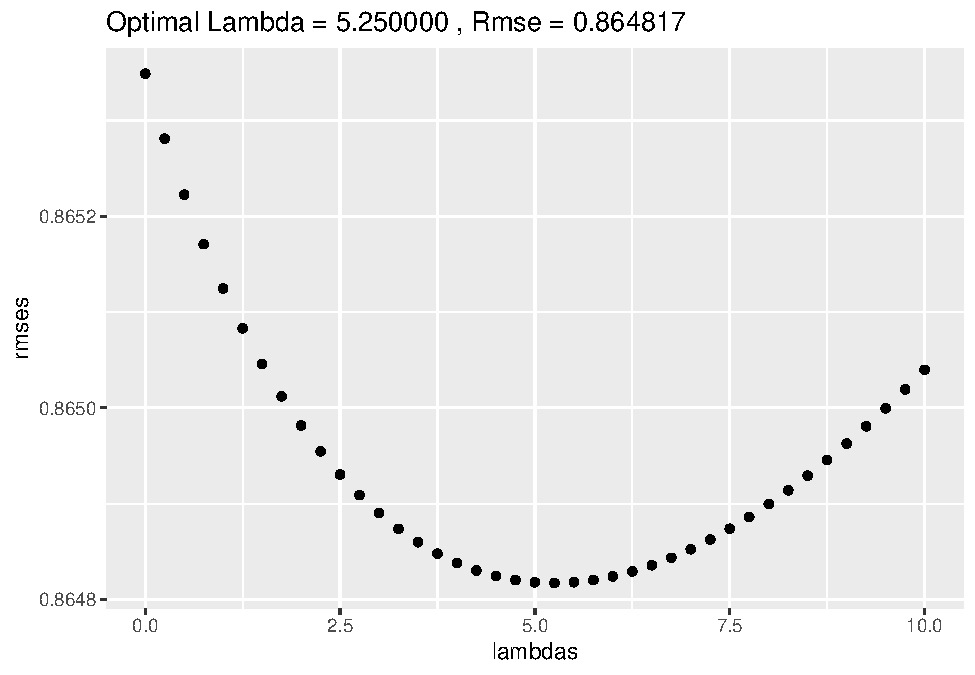
\includegraphics{Project_MovieLens_files/figure-latex/unnamed-chunk-29-1.pdf}

\begin{Shaded}
\begin{Highlighting}[]
\NormalTok{rmse_results <-}\StringTok{ }\KeywordTok{bind_rows}\NormalTok{(rmse_results,}
                          \KeywordTok{data_frame}\NormalTok{(}\DataTypeTok{method=}\StringTok{"Regularized movie and user effect model"}\NormalTok{,  }
                                     \DataTypeTok{RMSE =} \KeywordTok{min}\NormalTok{(rmses)))}
\end{Highlighting}
\end{Shaded}

\section{Results}
\label{sec:results}

In Section \ref{sec:methods}, we presented and discuss various models.
We started with a very simple model by predicting the mean regardless of
the user. Then, we realised that some movies are rated less compared to
popular movies. Moreover, some users love every movie and give a higher
rating to the movies. This led us to use movie and user effects with our
model to improve the performance. But small estimates can result in
overfitting of our model. Then, we use regularisation to produce a model
with the lowest RMSE.

\begin{Shaded}
\begin{Highlighting}[]
\NormalTok{rmse_results}
\end{Highlighting}
\end{Shaded}

\begin{longtable}[]{@{}lr@{}}
\toprule
method & RMSE\tabularnewline
\midrule
\endhead
Target RSME & 0.8649000\tabularnewline
Average Rating Model & 1.0612018\tabularnewline
Movie effect model & 0.9439087\tabularnewline
Movie and user effect model & 0.8653488\tabularnewline
Regularized movie and user effect model & 0.8648170\tabularnewline
\bottomrule
\end{longtable}

The RMSE of our best model is 0.8648170, which is lower than the
\textbf{Target RMSE}. This is also a significant improvement compared to
the first simple model i.e., around 18.5 \% decrease in RMSE.

\section{Conclusion}
\label{sec:conclusion}

In this report, we developed recommendation algorithms to predict movie
ratings using Movielens data. There is a lot of variability in our data,
such as popular movies are rated by many users, obscure movies have a
very low rating, some users like every movie, and some users give more
negative ratings. These factors prompted us to use average ratings of
movies and users with our model. We noticed a significant improvement to
the RMSE compared to our first model. Then, we used regularization to
handle the overfitting of our model and gained a slight increase in the
RMSE score.

\subsection{Future Work}
\label{sec:futurework}

We did not use the genre's information in our model. Maybe we can use
that in a future model by penalizing movies belonging to less common
genres. Similarly, we can compute the release year, which has the lowest
number of rated movies. Then, we can ignore movies from that year in our
model. But, we have to see the impact of these changes on the
performance of our model.

\begin{thebibliography}{9}
\bibitem{rsystems} 
Baptiste Rocca -Introduction to recommender systems \url{https://towardsdatascience.com/introduction-to-recommender-systems-6c66cf15ada}
\bibitem{rsystems1}
Resnick, P., Varian, H. \textit{Recommender Systems}. CACM 40(3), 56–58 (1997)
\bibitem{nfc}
Netflix Prize \url{https://en.wikipedia.org/wiki/Netflix_Prize}

\bibitem{dataset}
MovieLens 10M Dataset \url{https://grouplens.org/datasets/movielens/10m}

\bibitem{rmse}
James Moody - What does RMSE really mean? \url{https://towardsdatascience.com/what-does-rmse-really-mean-806b65f2e48e}

\bibitem{rafa}
Rafael Irizarry - Introduction to Data Science \url{https://rafalab.github.io/dsbook}


\end{thebibliography}


\end{document}
